%
% personal commentary:
%        DRAFT DRAFT DRAFT
%        - KFALL
% RNG section reviewed and revised 11-Sep-98, johnh.
%
% RNG section revised 28-Aug-02 by Tim Buchheim to include material
% from Michelle Weigle which describes the new implementation of RNG

\chapter{Mathematical Support}
\label{chap:math}

The simulator includes a small collection of mathematical
functions used to implement random variate generation and integration.
This area of the simulator is currently undergoing some
changes.

The procedures and functions described in this chapter can be found in
\nsf{tools/rng.\{cc, h\}},
\nsf{tools/random.\{cc, h\}},
\nsf{tools/ranvar.\{cc, h\}},
\nsf{tools/pareto.\{cc, h\}},
\nsf{tools/expoo.\{cc, h\}},
\nsf{tools/integrator.\{cc, h\}}, and
\nsf{tcl/lib/ns-random.tcl}.


\section{Random Number Generation}
\label{sec:random}

The RNG class contains an implementation of the combined multiple
recursive generator MRG32k3a proposed by L'Ecuyer
\cite{lecuyer99}. The C++ code was adapted from \cite{lecuyer01}.
This replaces the previous implementation of \code{RNG}, which used
the minimal standard multiplicative linear congruential generator of
Park and Miller~\cite{Park88:Random}.  The newer (MRG32k3a) \code{RNG} is
used in ns versions 2.1b9 and later.

The MRG32k3a generator provides $1.8$x$10^{19}$ independent
streams of random numbers, each of which consists of
$2.3$x$10^{15}$ substreams. Each substream has a period
(\emph{i.e.}, the number of random numbers before overlap) of
$7.6$x$10^{22}$. The period of the entire generator is
$3.1$x$10^{57}$. Figure \ref{streams} provides a graphical idea of
how the streams and substreams fit together.
\begin{figure}[ht]
\centering
\includegraphics[angle=270,width=6 in]{rng-streams.eps}
\caption{Overall arrangement of streams and substreams.
\cite{lecuyer01}} \label{streams}
\end{figure}

A default RNG ({\tt defaultRNG}), created at simulator initialization
time, is provided. If multiple random variables are used in a
simulation, each random variable should use a separate RNG object.
When a new RNG object is created, it is automatically seeded to
the beginning of the next independent stream of random numbers.
Used in this manner, the implementation allows for a maximum of
$1.8$x$10^{19}$ random variables.

Often, multiple independent replications of a simulation are
needed (\emph{i.e.}, to perform statistical analysis given
multiple runs with fixed parameters).  For each replication, a
different substream should be used to ensure that the random
number streams are independent. (This process is given as an OTcl
example later.) This implementation allows for a maximum of
$2.3$x$10^{15}$ independent replications. Each random variable in
a single replication can produce up to $7.6$x$10^{22}$ random
numbers before overlapping.

{\bf Note:} Only the most common functions are described here. For
more information, see \cite{lecuyer01} and the source code found
in {\tt tools/rng.h} and {\tt tools/rng.cc}.  For a comparison of this RNG to
the more common LCG16807 RNG (and why LCG16807 is not a good RNG), 
see \cite{lecuyer-wsc}.
\subsection{Seeding The RNG}
Due to the nature of the RNG and its implementation, it is not
necessary to set a seed (the default is 12345).  If you wish to
change the seed, functions are available. You should only set the
seed of the default RNG.  Any other RNGs you create are
automatically seeded such that they produce independent streams.
The range of valid seeds is 1 to {\tt MAXINT}.

To get non-deterministic behavior, set the seed of the default RNG
to 0.  This will set the seed based on the current time of day and
a counter.  {\bf This method should not be used to set seeds for
independent replications.}  There is no guarantee that the streams
produced by two random seeds will not overlap.  The only way to
guarantee that two streams do not overlap is to use the substream
capability provided by the RNG implementation.

\subsubsection{Example}
\begin{verbatim}
 # Usage: ns rng-test.tcl [replication number]

 if {$argc > 1} {
    puts "Usage: ns rng-test.tcl \[replication number\]"
    exit
 }
 set run 1
 if {$argc == 1} {
    set run [lindex $argv 0]
 }
 if {$run < 1} {
    set run 1
 }

 # seed the default RNG
 global defaultRNG
 $defaultRNG seed 9999

 # create the RNGs and set them to the correct substream
 set arrivalRNG [new RNG]
 set sizeRNG [new RNG]
 for {set j 1} {$j < $run} {incr j} {
    $arrivalRNG next-substream
    $sizeRNG next-substream
 }

 # arrival_ is a exponential random variable describing the time
 # between consecutive packet arrivals
 set arrival_ [new RandomVariable/Exponential]
 $arrival_ set avg_ 5
 $arrival_ use-rng $arrivalRNG

 # size_ is a uniform random variable describing packet sizes
 set size_ [new RandomVariable/Uniform]
 $size_ set min_ 100
 $size_ set max_ 5000
 $size_ use-rng $sizeRNG

 # print the first 5 arrival times and sizes
 for {set j 0} {$j < 5} {incr j} {
    puts [format "%-8.3f  %-4d" [$arrival_ value] \
            [expr round([$size_ value])]]
 }
\end{verbatim}

\subsubsection{Output}

\begin{verbatim}
 % ns rng-test.tcl 1
 6.358     4783
 5.828     1732
 1.469     2188
 0.732     3076
 4.002     626

 % ns rng-test.tcl 5
 0.691     1187
 0.204     4924
 8.849     857
 2.111     4505
 3.200     1143
\end{verbatim}

\subsection{OTcl Support}

\subsubsection{Commands}

The following commands on the RNG class can be accessed from OTcl
and are found in {\tt tools/rng.cc}:
\begin{description}
    \item[{\tt seed $n$}] -- seed the RNG to $n$, if $n == 0$, the seed
    is set according to the current time and a counter
    \item[{\tt next-random}] -- return the next random number
    \item[{\tt seed}] -- return the current value of the seed
    \item[{\tt next-substream}] -- advance to the next substream
    \item[{\tt reset-start-substream}] -- reset the stream to the beginning
    of the current substream
    \item[{\tt normal $avg$ $std$}] -- return a number sampled from a normal
    distribution with the given average and standard deviation
    \item[{\tt lognormal $avg$ $std$}] -- return a number sampled from a
      lognormal distribution with the given average and standard deviation
\end{description}

The following commands on the RNG class can be accessed from OTcl
and are found in {\tt tcl/lib/ns-random.tcl}:
\begin{description}
    \item[{\tt exponential $mu$}] -- return a number sampled from an
      exponential distribution with mean $mu$ 
    \item[{\tt uniform $min$ $max$}] -- return an integer sampled from a
    uniform distribution on [$min$, $max$]
    \item[{\tt integer $k$}] -- return an integer sampled from a uniform
    distribution on [0, $k$-1]
\end{description}

\subsubsection{Example}

\begin{verbatim}
 # Usage: ns rng-test2.tcl [replication number]

 if {$argc > 1} {
    puts "Usage: ns rng-test2.tcl \[replication number\]"
    exit
 }
 set run 1
 if {$argc == 1} {
    set run [lindex $argv 0]
 }
 if {$run < 1} {
    set run 1
 }

 # the default RNG is seeded with 12345

 # create the RNGs and set them to the correct substream
 set arrivalRNG [new RNG]
 set sizeRNG [new RNG]
 for {set j 1} {$j < $run} {incr j} {
    $arrivalRNG next-substream
    $sizeRNG next-substream
 }

 # print the first 5 arrival times and sizes
 for {set j 0} {$j < 5} {incr j} {
    puts [format "%-8.3f  %-4d" [$arrivalRNG lognormal 5 0.1] \
            [expr round([$sizeRNG normal 5000 100])]]
 }
\end{verbatim}

\subsubsection{Output}

\begin{verbatim}
 % ns rng-test2.tcl 1
 142.776   5038
 174.365   5024
 147.160   4984
 169.693   4981
 187.972   4982

 % ns rng-test2.tcl 5
 160.993   4907
 119.895   4956
 149.468   5131
 137.678   4985
 158.936   4871
\end{verbatim}

\subsection{C++ Support}

\subsubsection{Member Functions}
The random number generator is implemented by the RNG class and is
defined in {\tt tools/rng.h}.

{\bf Note:} The Random class in {\tt tools/random.h} is an older
interface to the standard random number stream.

Member functions provide the following operations:

\begin{description}
    \item[{\tt void set\_seed (long seed)}] -- set the seed of the RNG, if
    $seed == 0$, the seed is set according to the current time and a
    counter
    \item[{\tt long seed (void)}] -- return the current seed
    \item[{\tt long next (void)}] -- return the next random number as an
    integer on [0, {\tt MAXINT}]
    \item[{\tt double next\_double (void)}] -- return the next random number
    on [0, 1]
    \item[{\tt void reset\_start\_substream (void)}] -- reset the stream
    to the beginning of the current substream
    \item[{\tt void reset\_next\_substream (void)}] -- advance to the next
    substream
    \item[{\tt int uniform (int k)}] -- return an integer sampled from a
      uniform distribution on [0, k-1]
    \item[{\tt double uniform (double r)}] -- return a number sampled from a
      uniform distribution on [0, r]
    \item[{\tt double uniform (double a, double b)}] -- return a number
      sampled from a uniform distribution on [a, b]
    \item[{\tt double exponential (void)}] -- return a number sampled from an
    exponential distribution with mean 1.0
    \item[{\tt double exponential (double k)}] -- return a number sampled from
      an exponential distribution with mean k 
    \item[{\tt double normal (double avg, double std)}] -- return a number
      sampled from a normal distribution with the given average and standard 
    deviation
    \item[{\tt double lognormal (double avg, double std)}] -- return a number
      sampled from a lognormal distribution with the given average and
      standard deviation
\end{description}

\subsubsection{Example}

\begin{verbatim}
 /* create new RNGs */
 RNG arrival (23456);
 RNG size;

 /* set the RNGs to the appropriate substream */
 for (int i = 1; i < 3; i++) {
   arrival.reset_next_substream();
   size.reset_next_substream();
 }

 /* print the first 5 arrival times and sizes */
 for (int j = 0; j < 5; j++) {
   printf ("%-8.3f  %-4d\n", arrival.lognormal(5, 0.1),
             int(size.normal(500, 10)));
 }
\end{verbatim}

\subsubsection{Output}
\begin{verbatim}
 161.826   506
 160.591   503
 157.145   509
 137.715   507
 118.573   496
\end{verbatim}





\section{Random Variables}
\label{sec:ranvar}

The \clsref{RandomVariable}{../ns-2/ranvar.h}
provides a thin layer of functionality on top
of the base random number generator and the default random number stream.
It is defined in \nsf{ranvar.h}:

\begin{program}
  class RandomVariable : public TclObject \{
  public:
        virtual double value() = 0;
        int command(int argc, const char*const* argv);
        RandomVariable();
  protected:
        RNG* rng_;
  \};
\end{program}

Classes derived from this abstract class implement specific
distributions.  Each distribution is parameterized with the values of
appropriate parameters.  The value method is used to return a value
from the distribution.  

The currently defined distributions, and their associated parameters are:

\begin{tabular}{rl}
\clsref{UniformRandomVariable}{tools/ranvar.h} & \code{min_}, \code{max_} \\
\clsref{ExponentialRandomVariable}{tools/ranvar.h} & \code{avg_} \\
\clsref{ParetoRandomVariable}{tools/ranvar.h} & \code{avg_}, \code{shape_}\\
\clsref{ParetoIIRandomVariable}{tools/ranvar.h} & \code{avg_}, \code{shape_}\\
\clsref{ConstantRandomVariable}{tools/ranvar.h} & \code{val_}\\
\clsref{HyperExponentialRandomVariable}{tools/ranvar.h} & \code{avg_}, \code{cov_}\\
\clsref{NormalRandomVariable}{tools/ranvar.h} & \code{avg_}, \code{std_}\\
\clsref{LogNormalRandomVariable}{tools/ranvar.h} & \code{avg_}, \code{std_}\\
\end{tabular}

The RandomVariable class is available in OTcl.  For instance, to
create a random variable that generates number uniformly on [10, 20]:
\begin{program}
        set u [new RandomVariable/Uniform]
        $u set min_ 10
        $u set max_ 20
        $u value
\end{program}
By default, RandomVariable objects use the default random number
generator described in the previous section.  The use-rng method can
be used to associate a RandomVariable with a non-default RNG:
\begin{program}
        set rng [new RNG]
        $rng seed 0

        set e [new RandomVariable/Exponential]
        $e use-rng $rng
\end{program}


\section{Integrals}
\label{sec:integral}

The  \clsref{Integrator}{../ns-2/integrator.h}
supports the approximation of (continuous) integration by (discrete)
sums; it is defined in \nsf{integrator.h} as
\begin{program}
{\rm From integrator.h:}
        class Integrator : public TclObject \{
        public:
                Integrator();
                void set(double x, double y);
                void newPoint(double x, double y);
                int command(int argc, const char*const* argv);
        protected:
                double lastx_;
                double lasty_;
                double sum_;
        \};

{\rm From integrator.cc:}
        Integrator::Integrator() : lastx_(0.), lasty_(0.), sum_(0.)
        \{
                bind("lastx_", &lastx_);
                bind("lasty_", &lasty_);
                bind("sum_", &sum_);
        \}

        void Integrator::set(double x, double y)
        \{
                lastx_ = x;
                lasty_ = y;
                sum_ = 0.;
        \}

        void Integrator::newPoint(double x, double y)
        \{
                sum_ += (x - lastx_) * lasty_;
                lastx_ = x;
                lasty_ = y;
        \}

        int Integrator::command(int argc, const char*const* argv)
        \{
                if (argc == 4) \{
                        if (strcmp(argv[1], "newpoint") == 0) \{
                                double x = atof(argv[2]);
                                double y = atof(argv[3]);
                                newPoint(x, y);
                                return (TCL_OK);
                        \}
                \}
                return (TclObject::command(argc, argv));
        \}
\end{program}
This class provides a base class used by other classes such
as \code{QueueMonitor} that keep running sums.
Each new element of the running sum is added by
the \fcn[x, y]{newPoint} function.
After the $k$th execution of \code{newPoint}, the running sum
is equal to $\sum_{i=1}^{k}y_{i-1}(x_i - x_{i-1})$ where
$x_0 = y_0 = 0$ unless \code{lastx\_}, \code{lasty\_}, or \code{sum\_}
are reset via OTcl.
Note that a new point in the sum can be added either by the
C++ member \code{newPoint} or the OTcl member \code{newpoint}.
The use of integrals to compute certain types of averages
(e.g. mean queue lengths) is given in (pp. 429--430, \cite{Jain91:Art}).

\section{\code{ns-random}}

{\bf \code{ns-random} is an obsolete way to generate random numbers. 
This information is provided only for backward compatibility.}

\code{ns-random} is implemented in \nsf{misc.\{cc,h\}}. 
When called with no argument, it generates a random number with
uniform distribution between 0 and \code{MAXINT}.
When an integer argument is provided, it seeds the random generater
with the given number.
A special case is when \code{ns-random 0} is called, it randomly seeds
the generator based on current time.
This feature is useful to produce non-deterministic results across
runs.

\section{Some mathematical-support related objects}
\label{sec:mathobjects}

\textsc{Integrator objects}
Integrator Objects support the approximate computation of continuous
integrals using discrete sums. The running sum(integral) is computed as:
\code{sum_ += [lasty_ * (x lastx_)]} where (x, y) is the last element
entered and
(lastx\_, lasty\_) was the element previous to that added to the sum.
lastx\_ and lasty\_ are updated as new elements are added. The first
sample point defaults to (0,0) that can be changed by changing the values
of (lastx\_,lasty\_). 
\code{$integrator newpoint <x> <y>}\\ %$
Add the point (x,y) to the sum. Note that it does not make sense for x to
be less than lastx\_. 

There are no configuration parameters specific to this object. \\

State Variables are:
\begin{description}
\item[lastx\_]
x-coordinate of the last sample point. 

\item[lasty\_]
y-coordinate of the last sample point. 

\item[sum\_] Running sum (i.e. the integral) of the sample points. 
\end{description}


\textsc{Samples Object}
Samples Objects support the computation of mean and variance statistics
for a given sample. 

\code{$samples mean}\\
Returns mean of the sample. 

\code{$samples variance}\\
Returns variance of the sample. 

\code{$samples cnt}\\
Returns a count of the sample points considered. 

\code{$samples reset }\\
Reset the Samples object to monitor a fresh set of samples. 

There are no configuration parameters or state variables specific to this
object. 



\section{Commands at a glance}
\label{sec:mathcommand}

Following is a list of mathematical support related commands commonly used
in simulation scripts:
\begin{flushleft}
\code{set rng [new RNG]}\\
This creates a new random number generator.


\code{$rng seed <0 or n>}\\
This command seeds the RNG. If 0 is specified, the RNG is seeded
heuristically. Otherwise the RNG is seeded with the value <n>.


\code{$rng next-random}\\
This returns the next random number from RNG.


\code{$rng uniform <a> <b>}\\
This returns a number uniformly distributed on <a> and <b>.


\code{$rng integer <k>}\\
This returns an integer uniformly distributed on 0 and k-1.


\code{$rng exponential}\\
This returns a number that has exponential distribution with average 1.


\code{set rv [new Randomvariable/<type of random-variable>]}\\
This creates an instance of a random variable object that generates random 
variables with specific distribution. The different types of random 
variables derived from the base class are:\\
RandomVariable/Uniform, RandomVariable/Exponential, RandomVariable/Pareto,
RandomVariable/Constant, RandomVariable/HyperExponential.
Each of these distribution types are parameterized with values of
appropriate parameters. For details see section \ref{sec:ranvar} of this
chapter.


\code{$rv use-rng <rng>}\\
This method is used to associated a random variable object with a
non-default RNG. Otherwise by default, the random variable object is
associated with the default random number generator.


\end{flushleft}




% LocalWords:  ranvar pareto expoo tcl lib ns cc integrator RNG rng TclObject
% LocalWords:  enum RNGSources PREDEF int MAXINT rX edv prob edp setbit iph ECN
% LocalWords:  ip ecn eed OURCE OTcl RandomVariable argc const argv min avg val
% LocalWords:  UniformRandomVariable ExponentialRandomVariable cov newPoint pp
% LocalWords:  ParetoRandomVariable ConstantRandomVariable lastx lasty strcmp
% LocalWords:  HyperExponentialRandomVariable newpoint atof QueueMonitor
